% The primary readability contrast as a forest.
% Chapter 4, Section 4.3.2, beside Table~\ref{tab:readability-conditioning},
% which it draws.
%
% Drawn by scripts/figureread.py, which reads the effects and intervals out of
% tables/main/readability_02_conditioning.csv rather than recomputing them, so
% this figure and that table are one result drawn twice. The script refuses to
% run if the file is absent.
%
% Drawn on the 9.0 inch canvas and set at 15.7 points, so the type arrives at 11
% points once this is included at \textwidth. Include at \textwidth and do not
% scale.
%
% Caption text is config/captions.yml under readability_conditioning.
\begin{figure}[htbp]
\centering
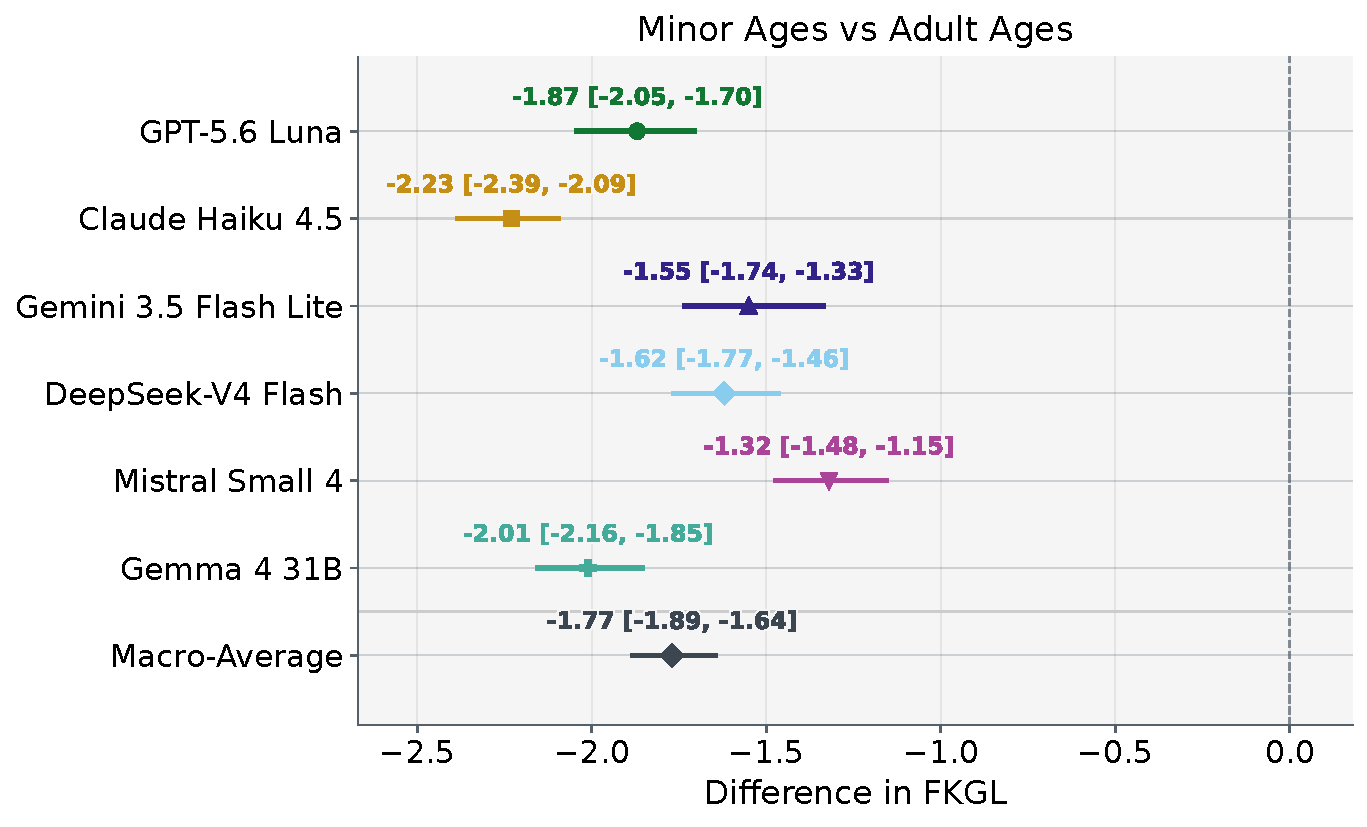
\includegraphics[width=\textwidth]{read/readability_conditioning.pdf}
\caption[The Primary Readability Contrast]{The primary readability contrast from
Table~\ref{tab:readability-conditioning}, one row a model, in school grades with
95\% bootstrap intervals, paired within scenario. A negative effect is a reply to
an explicit minor age sitting at a lower grade level than one to an explicit
adult age on the same scenario. Only scenarios complete across all eight explicit
ages enter, so the denominator differs by model and is given in that table. The
macro-average is the mean of the six effects under a joint bootstrap that
resamples the scenario set once and applies the draw to every model, so its
interval carries the dependence between models sharing scenarios. It sits below
the rule because it summarises the six rows and is not a seventh model.}
\label{fig:readability-conditioning}
\end{figure}
